\tikzstyle{block} = [draw, fill=blue!0, rectangle, 
    minimum height=2.5em, minimum width=5em,align=center]
\tikzstyle{block2} = [draw, fill=blue!0, rectangle, 
    minimum height=5em, minimum width=8em,align=center]
\tikzstyle{sum} = [draw, fill=blue!0, circle, node distance=1cm]
\tikzstyle{input} = [coordinate]
\tikzstyle{tmp} = [coordinate]
\tikzstyle{output} = [coordinate]
\tikzstyle{pinstyle} = [pin edge={to-,thin,black}]
\tikzset{
  image/.style={
    path picture={
      \node[anchor=center] at (path picture bounding box.center) {
        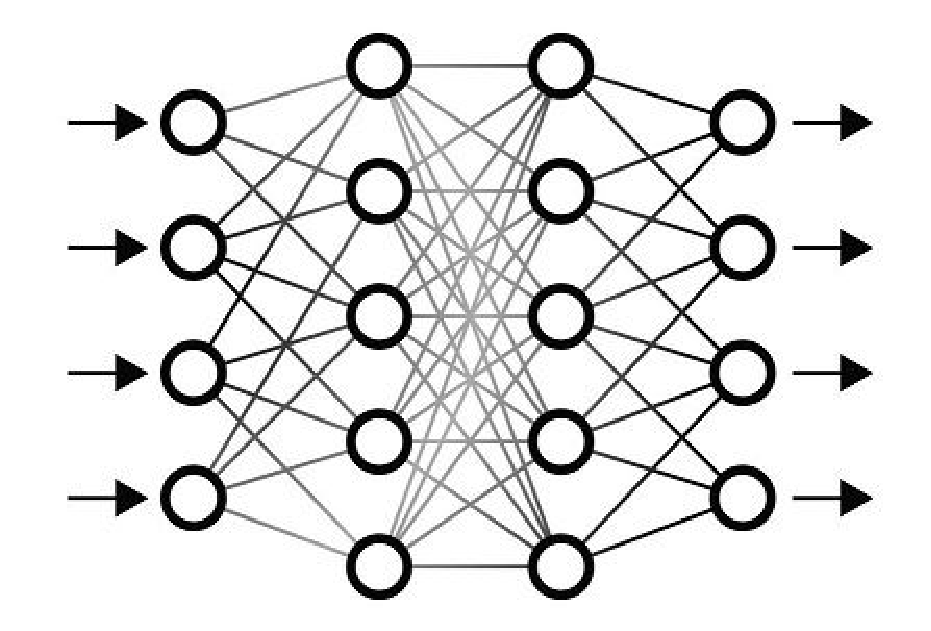
\includegraphics[width=2.5cm]{figures/AI/neural-network-icon.pdf}};}}
  }
\begin{tikzpicture}[auto, node distance=2cm,>=latex']
% Boxing and labelling noise shapers
	\draw [color=black,thick,fill={rgb:black,1;white,30}](7.5,1.2) rectangle (12.4,-0.8);
	\node at (7.5,0.9) [below=1mm, right=2mm] {{Spacecraft Bus}};

    \node [input, name=input] {};
    \node [sum, right of=input](sum) {};
    \node [block, right of=sum, name=ctrl,node distance=1.5cm]
        {Control \\ Law};
    \node [block2,  color=white,image, right of=ctrl, name=str,node distance=3.1cm]
        {};
    \node at (4,1) [above=10mm, right=4mm] {{NN Steering}};
	
    \node [block, right of=str,node distance=3.1cm] (cmg)
        {VSCMG \\ Cluster};
    \node [block, right of=cmg,node distance=2.5cm] (sys)
        {Platform \\ Dynamics};
    \node [output,right of=sys,node distance=2cm] (output){};
    
    
    \draw [draw,->] (input) -- node[anchor=south east] {$q_d,\omega_d$} (sum);
    \draw[->](sum)--node {$e$}(ctrl);
    \draw[->](ctrl)--node {$\tau_c$}(str);
    \draw[->](str)--node[anchor=south east] {$ \ \dot{\delta} $}node[anchor=north east] {$ \ \dot{\Omega}$}(cmg);
    \draw[->](cmg)--node {$\tau_{a}$}(sys);
    \draw[->](sys)-- node [name=y] {$q,\omega$}(output);
    \node[tmp,below of=sys,node distance=1.5cm](fo1){};
    \node[tmp,below of=y,node distance=2.5cm](fo2){};
    \draw[->](y)--(fo2)-|node[pos=0.99] {$-$} 
        node [near start] {Spacecraft Quaternion and body rate feedback ($q,\omega$)}(sum);
    \draw[->](sys)--(fo1)-|node [near start] {VSCMG State feedback ($\delta,\Omega$)}(str);


\end{tikzpicture}